
\part{无监督学习}

\section{聚类}

\subsection{k均值}
k均值(k-means)是一种是硬聚类算法,其工作流程如下: \\\indent随机选择k个点作为初始质心(质心即簇中所有点的中心),然后将数据集中的每个点分配到一个簇中,具体来讲,为每个点找距其最近的质心,并将其分配给该质心所对应的簇。这一步完成之后,每个簇的质心更新为该簇所有点的平均值。重复以上步骤,直到质心不发生变化。我理解其工作流程为实质为\textcolor{red}{利用推广的坐标下降算法(多变量)将目标函数极小化}。

\subsubsection{k均值算法}

\noindent\textbf{K均值算法流程:}
\begin{figure}[!h]
  \centering
  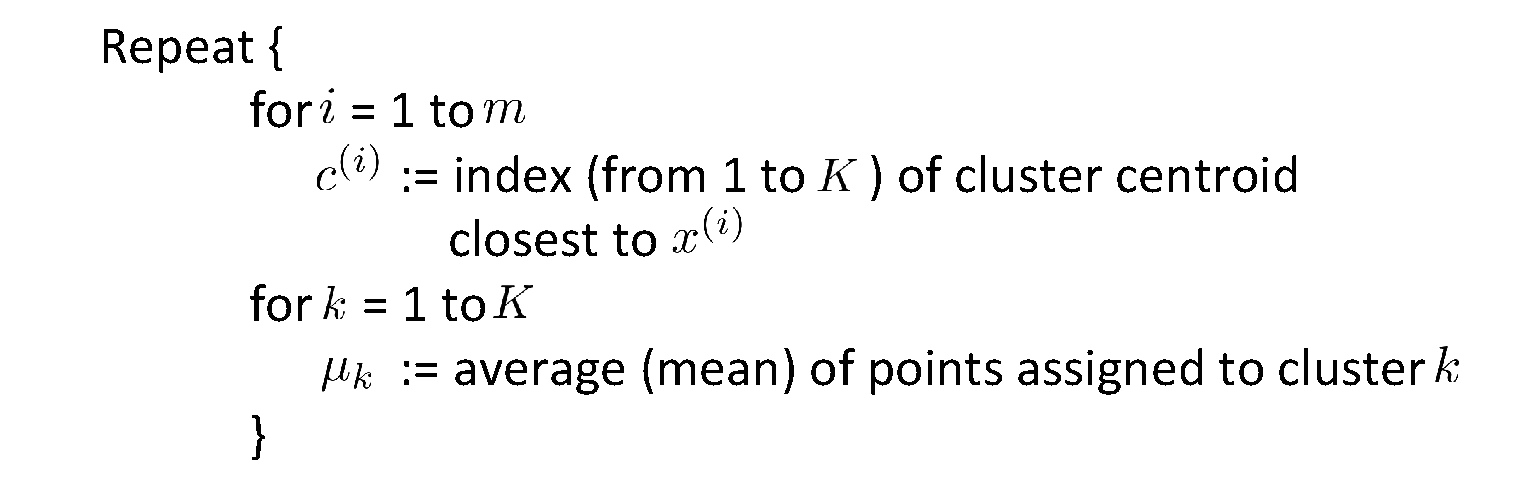
\includegraphics[width=0.8\textwidth]{KM.eps}
\end{figure}

\subsubsection{距离度量}
特征空间中两个实例点的距离是两个实例点相似程度的反映。k近邻模型的特征空间一般是n维实数向量空间$~R^n~$,使用的距离是欧氏距离,但也可以是其他距离, 如更一般的$~L_p~$距离$~(L_p~distance)~$或~Minkowski~距离(Minkowski~distance)。
\begin{align}
    L_p\text{距离}&: \nonumber\\
    &L_p(x_i,x_j)=\Big(\sum_{l=1}^{n}|x_i^{(l)}-x_j^{(l)}|^p\Big)^{\frac{1}{p}} \nonumber \\
    p=1~~~&\text{曼哈顿距离}:\nonumber \\
    &L_1(x_i,x_j)=\Big(\sum_{l=1}^{n}|x_i^{(l)}-x_j^{(l)}|\Big) \nonumber \\
    p=2~~~&\text{欧氏距离}:\nonumber\\
    &L_2(x_i,x_j)=\Big(\sum_{l=1}^{n}|x_i^{(l)}-x_j^{(l)}|^2\Big)^{\frac{1}{2}} \nonumber \\
    p=\infty~&~:\nonumber\\
    &L_\infty(x_i,x_j)=\max\limits_l |x_i^{(l)}-x_j^{(l)}| \nonumber
\end{align}

显然\textcolor{red}{不同的距离度量所确定的最近邻点是不同的}。


\subsubsection{K均值算法的优化目标}
\noindent
$c^{(i)}~$:当前第i个样本所属类别;\\
$\mu_k~$:第k的聚类中心的位置;\\
$\mu_c(i)~$:$x^{(i)}$所属族的聚类中心;\\
\textcolor{red}{Loss Function:}\\
$$J(c^{(1)},c^{(2)},...,c^{(m)},\mu_1,\mu_2,\mu_K)=\frac{1}{m}\sum_{i=1}^{m}||x^{(i)}-\mu_c(i)||^2$$

k-means
\begin{align}
            &\min \limits_{c^{(1,..,m),\mu_{1,..,K}}}~J(c^{(1)},c^{(2)},...,c^{(m)},\mu_1,\mu_2,\mu_K)  \nonumber
\end{align}

事实上从这就可以看出 k均值算法 的两部循环就是坐标下降算法推广分别固定类中心和样本点两类变量,来极小化损失函数。

\subsubsection{算法优点以及问题}
\noindent \textbf{优点:}\\
\indent 1.算法快速、简单;\\
\indent 2.对大数据集有较高的效率并且是可伸缩性的;\\
\indent 3.时间复杂度近于线性,而且适合挖掘大规模数据集。时间复杂度是O(nkt) ,其中n代表数据集中对象的数量,t代表着算法迭代的次数,k代表着簇的数目。\\


\noindent\textbf{1.偶尔陷入局部最优解}

解决方案:\\
\indent 1.随机初始化
\begin{figure}[!ht]
  \centering
  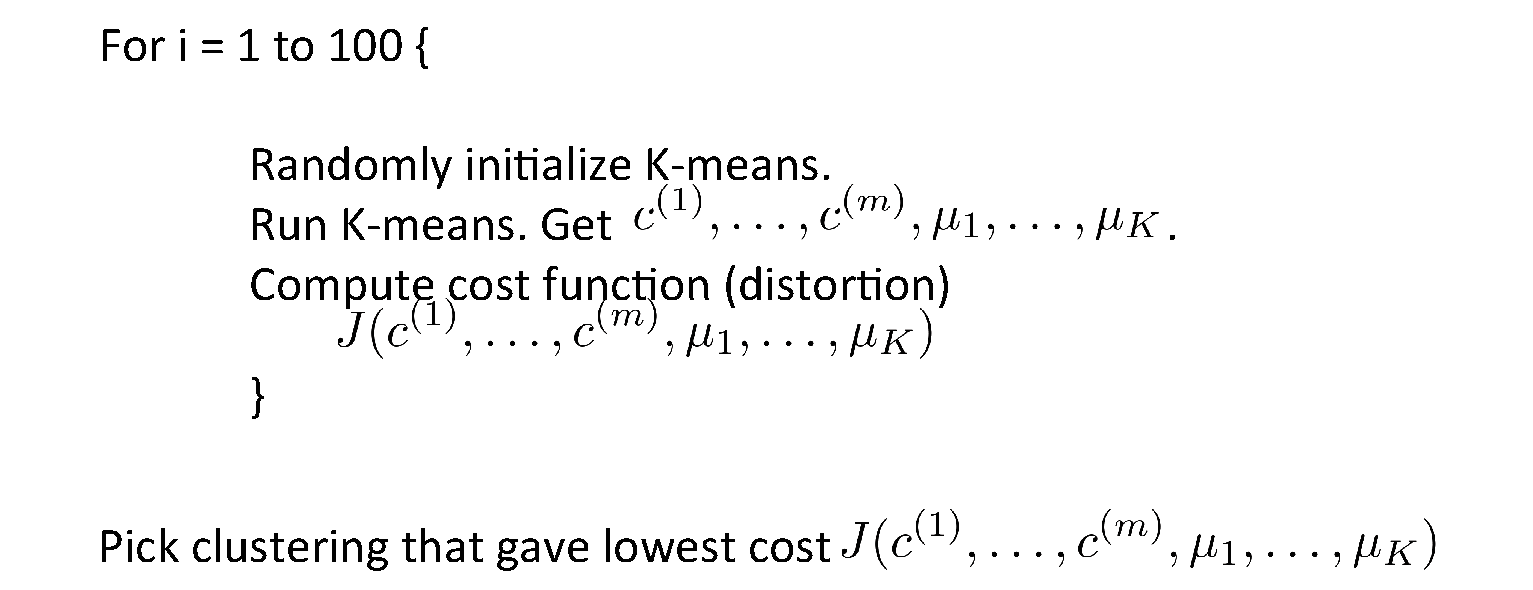
\includegraphics[width=0.8\textwidth]{RI.eps}
\end{figure}

\textcolor{red}{2.层次聚类(二分k均值)}


\noindent\textbf{2.聚类数目K值难以确定}

解决方案:\\
\indent 1.Elbow method(肘部法则)  \\
\indent 2.实际目的(聚类往往伴随着实际问题)


\subsubsection{实现K均值算法}
\noindent\textbf{核心函数}
\begin{lstlisting}
def kMeans(dataSet, k, distMeas=distEclud, createCent=randCent):
    m = shape(dataSet)[0]
    clusterAssment = mat(zeros((m,2)))#create mat to assign data points
                                      #to a centroid, also holds SE of each point
    centroids = createCent(dataSet, k)
    clusterChanged = True
    while clusterChanged:
        clusterChanged = False
        for i in range(m):#for each data point assign it to the closest centroid
            minDist = inf; minIndex = -1
            for j in range(k):
                distJI = distMeas(centroids[j,:],dataSet[i,:])
                if distJI < minDist:
                    minDist = distJI; minIndex = j
            if clusterAssment[i,0] != minIndex: clusterChanged = True
            clusterAssment[i,:] = minIndex,minDist**2
        print centroids
        for cent in range(k):#recalculate centroids
            ptsInClust = dataSet[nonzero(clusterAssment[:,0].A==cent)[0]]#get all the point in this cluster
            centroids[cent,:] = mean(ptsInClust, axis=0) #assign centroid to mean
    return centroids, clusterAssment
\end{lstlisting}

\newpage
\noindent 运行结果可视化:
\begin{figure}[h]
  \centering
  \includegraphics[width=0.8\textwidth]{KMeans.eps}
\end{figure}






